% !TeX spellcheck = en_US
\documentclass[french]{yLectureNote}

\title{Atomistique 2 - PS}
\subtitle{Chimie}
\author{Paulhenry Saux}
\date{\today}
\yLanguage{Français}

\professor{J.Cunny}
\usepackage{graphicx}%----pour mettre des images
\usepackage[utf8]{inputenc}%---encodage
\usepackage{geometry}%---pour modifier les tailles et mettre a4paper
%\usepackage{awesomebox}%---pour les boites d'exercices, de pbq et de croquis ---d\'esactiv\'e pour les TP de PC
\usepackage{tikz}%---pour deiffner + d\'ependance de chemfig
% \usepackage{tabularx}%---pour dimensionner automatiquement les tableaux avec variable X
\usepackage{awesomebox}%---Pour les boites info, danger et autres
\usepackage{menukeys}%---Pour deiffner les touches de Calculatrice
\usepackage{fancyhdr}%---pour les en-t\^ete personnalis\'ees
\usepackage{blindtext}%---pour les liens
\usepackage{hyperref}%---pour les liens (\`a mettre en dernier)
\usepackage{caption}%---pour la francisation de la l\'egende table vers Tableau
\usepackage{pifont}
\usepackage{array}%---pour les tableaux
\usepackage{lipsum}
\usepackage{yFlatTable}
\usepackage{multicol}
\newcommand{\Lim}[1]{\lim\limits_{\substack{#1}}\:}
\renewcommand{\vec}{\overrightarrow}
\newcommand{\N}[0]{\mathbb{N}}
\newcommand{\dd}{\mathrm{d}}
\newcommand{\norm}[1]{||\vec{#1}||}
\newcommand{\fo}{\psi(\vec{r},t)}
\newcommand{\foe}{\psi(\vec{r},t)\*}
\newcommand{\HH}{\hat{H}}
\newcommand{\hb}{\hbar}
\newcommand{\lap}{\nabla^2}
\newcommand{\lapcc}{\frac{\partial^2 }{\partial x^2}+\frac{\partial^2 }{\partial y^2}+\frac{\partial^2 }{\partial z^2}}
\begin{document}
\setcounter{chapter}{1}
\chapter{Orbitales moléculaires}
\section{Diagrammes à connaitre simples}
Diagramme HeH :

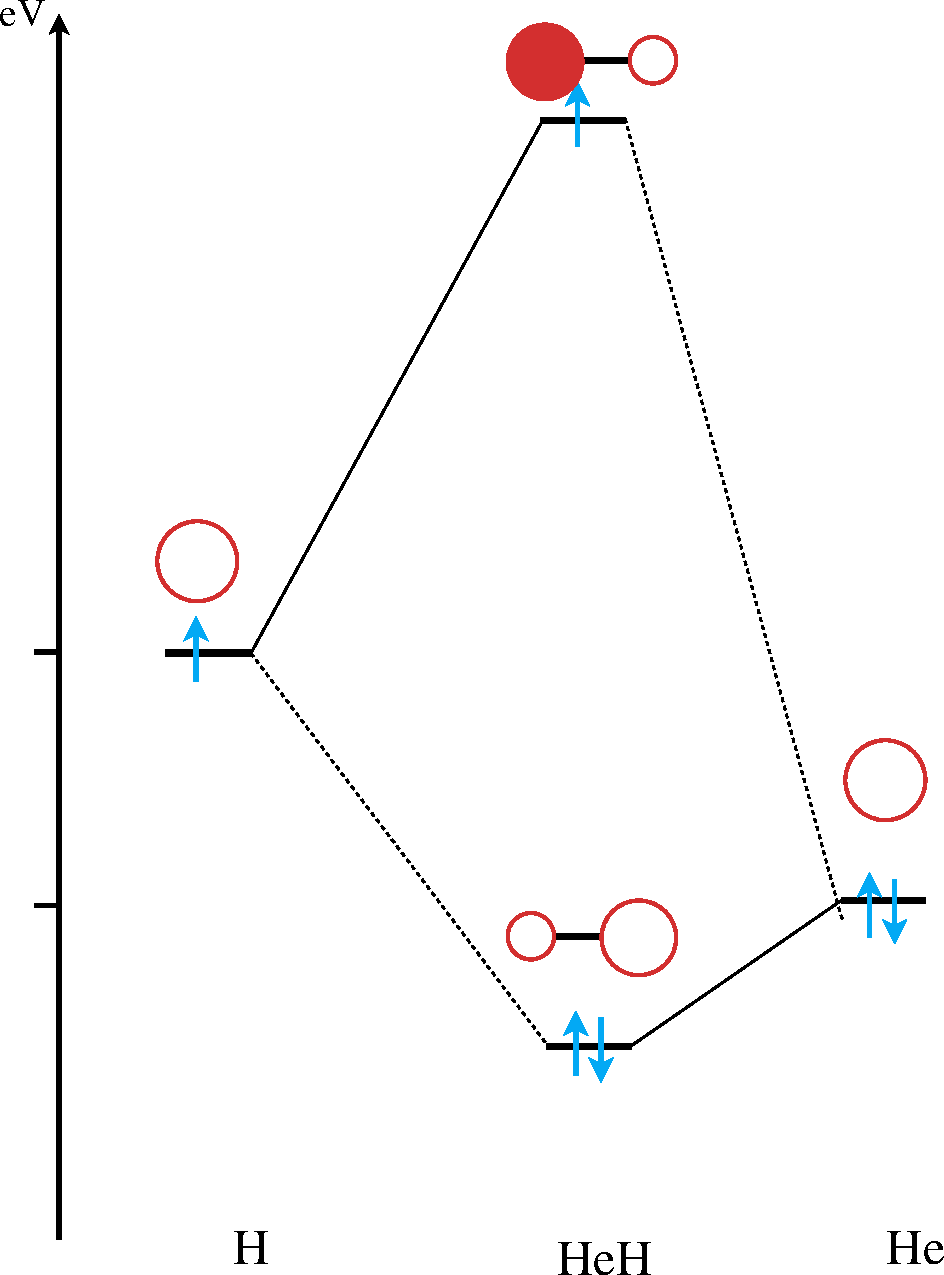
\includegraphics[scale=0.5]{figures/DOM_HeH}

Diagramme LiH :

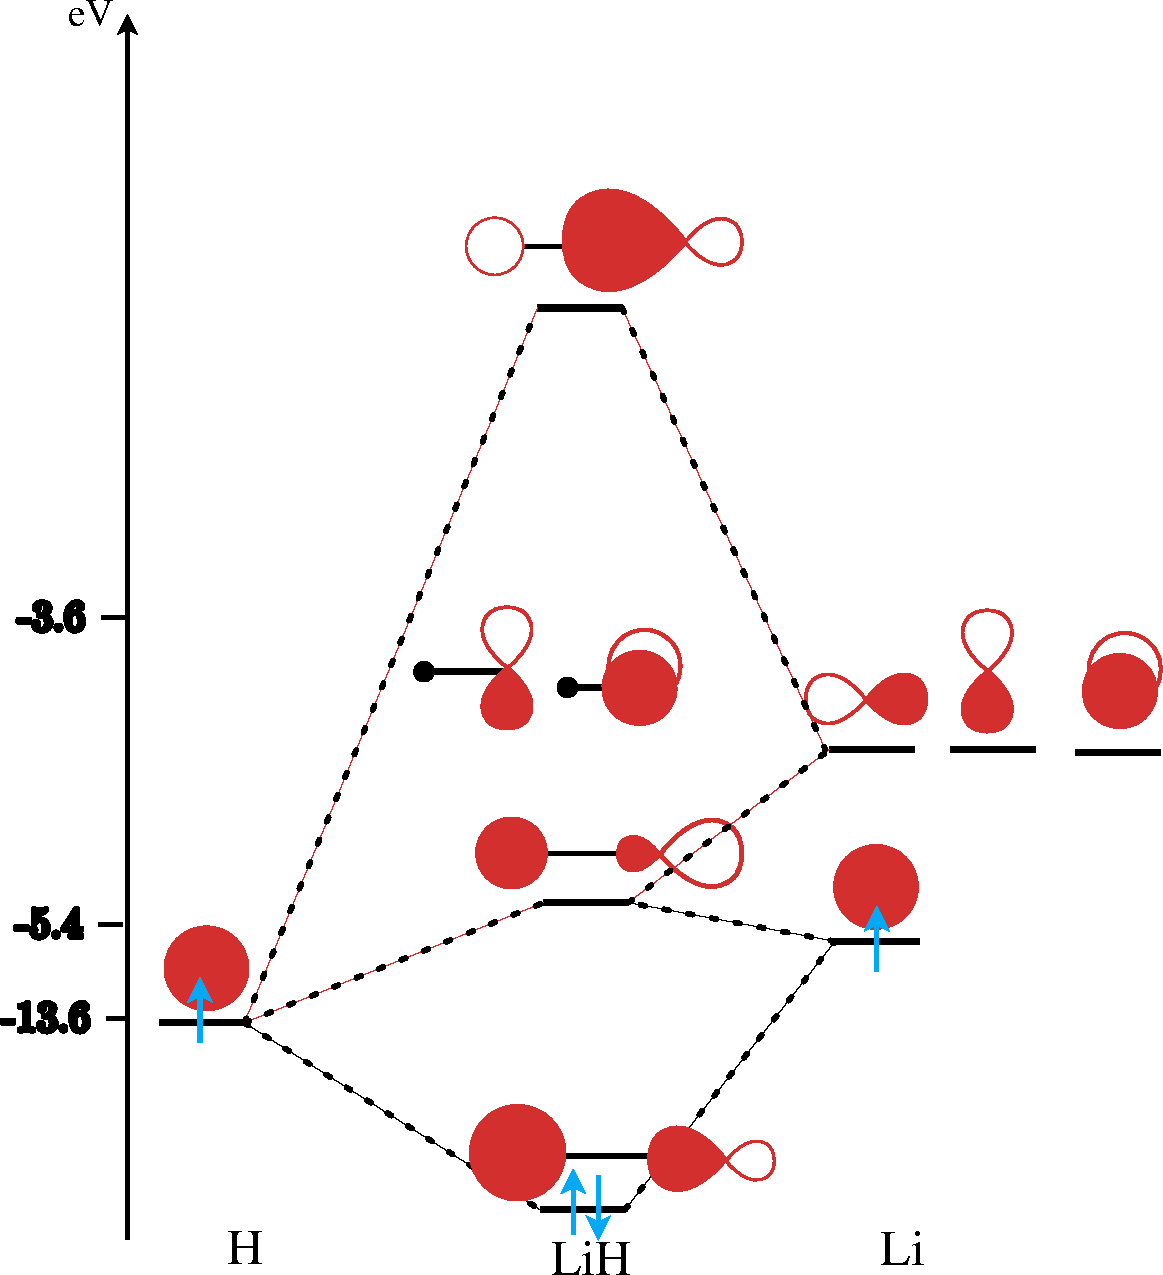
\includegraphics[scale=0.5]{figures/DOM_LIh}

Diagramme FH :

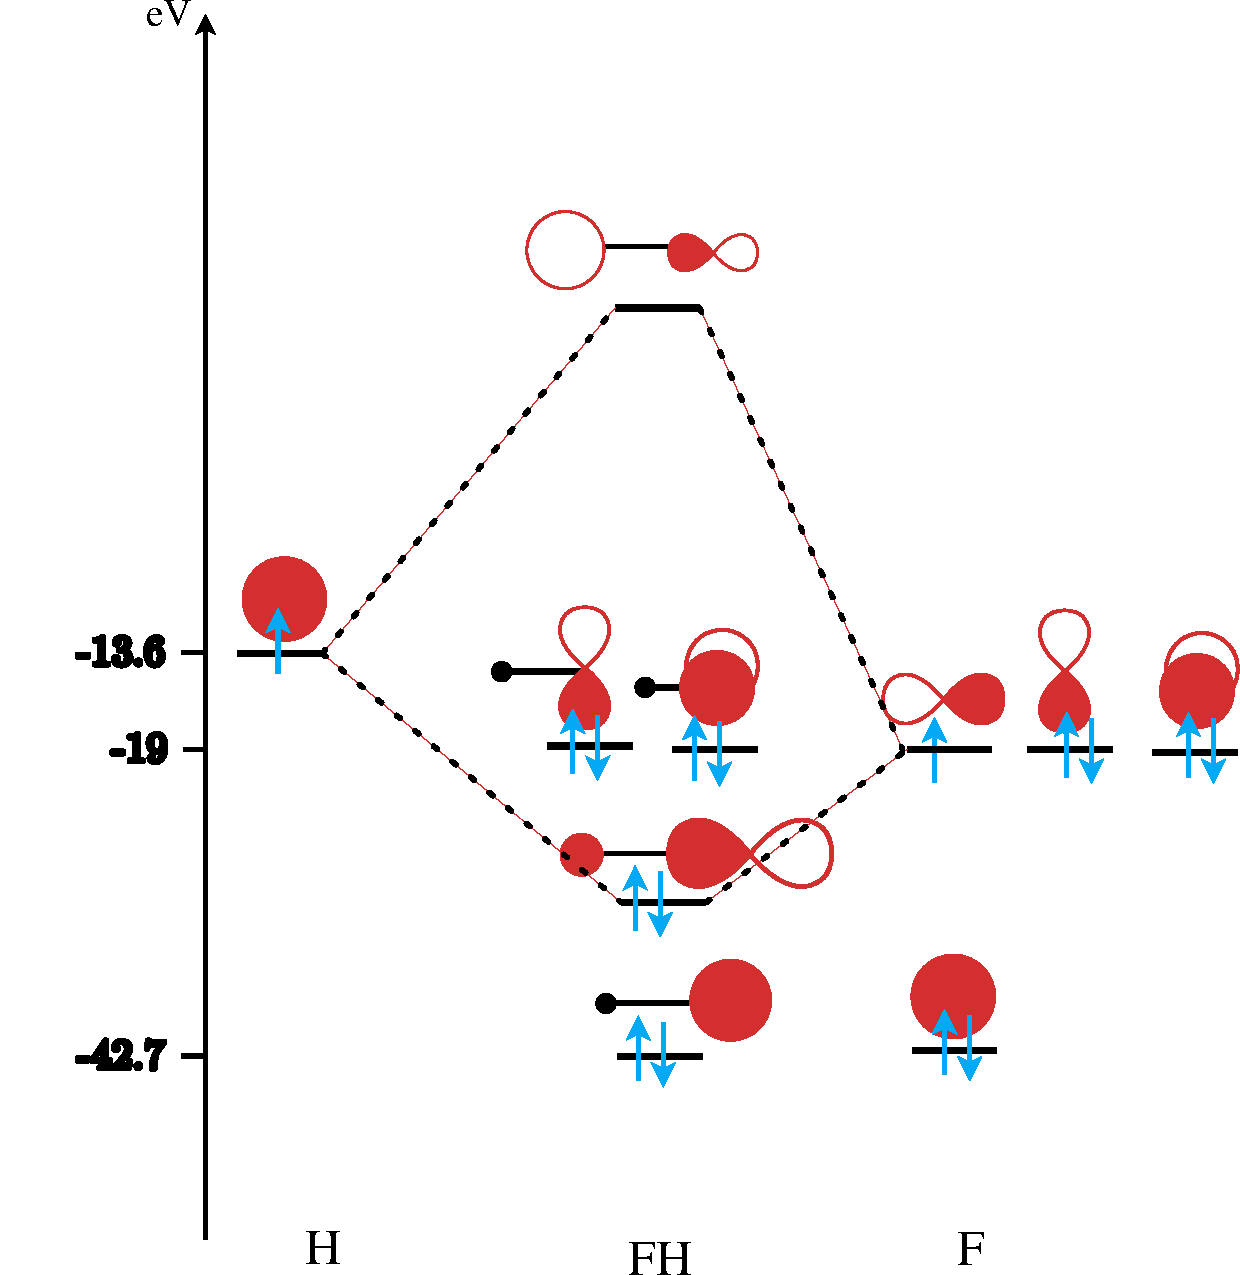
\includegraphics[scale=0.5]{figures/DOM_FH}
\section{Diagramme complexes}

\subsubsection{Avec fragmentation}
On peut séparer en HBe + H ou en HH + Be. Comme on veut conserver la symétrie de la molécule, on prend la seconde séparation. On va donc faire le DOM avec les OA de Be et les OM de $H_2$. On obtient\marginTips{On indique avec la lettre u ou g en indice si l'OM possède un centre de symétrie ou un centre d'anti-symétrie. On note AL les OM anti-liantes, NL les OM non-liantes, et L les OM liantes} :

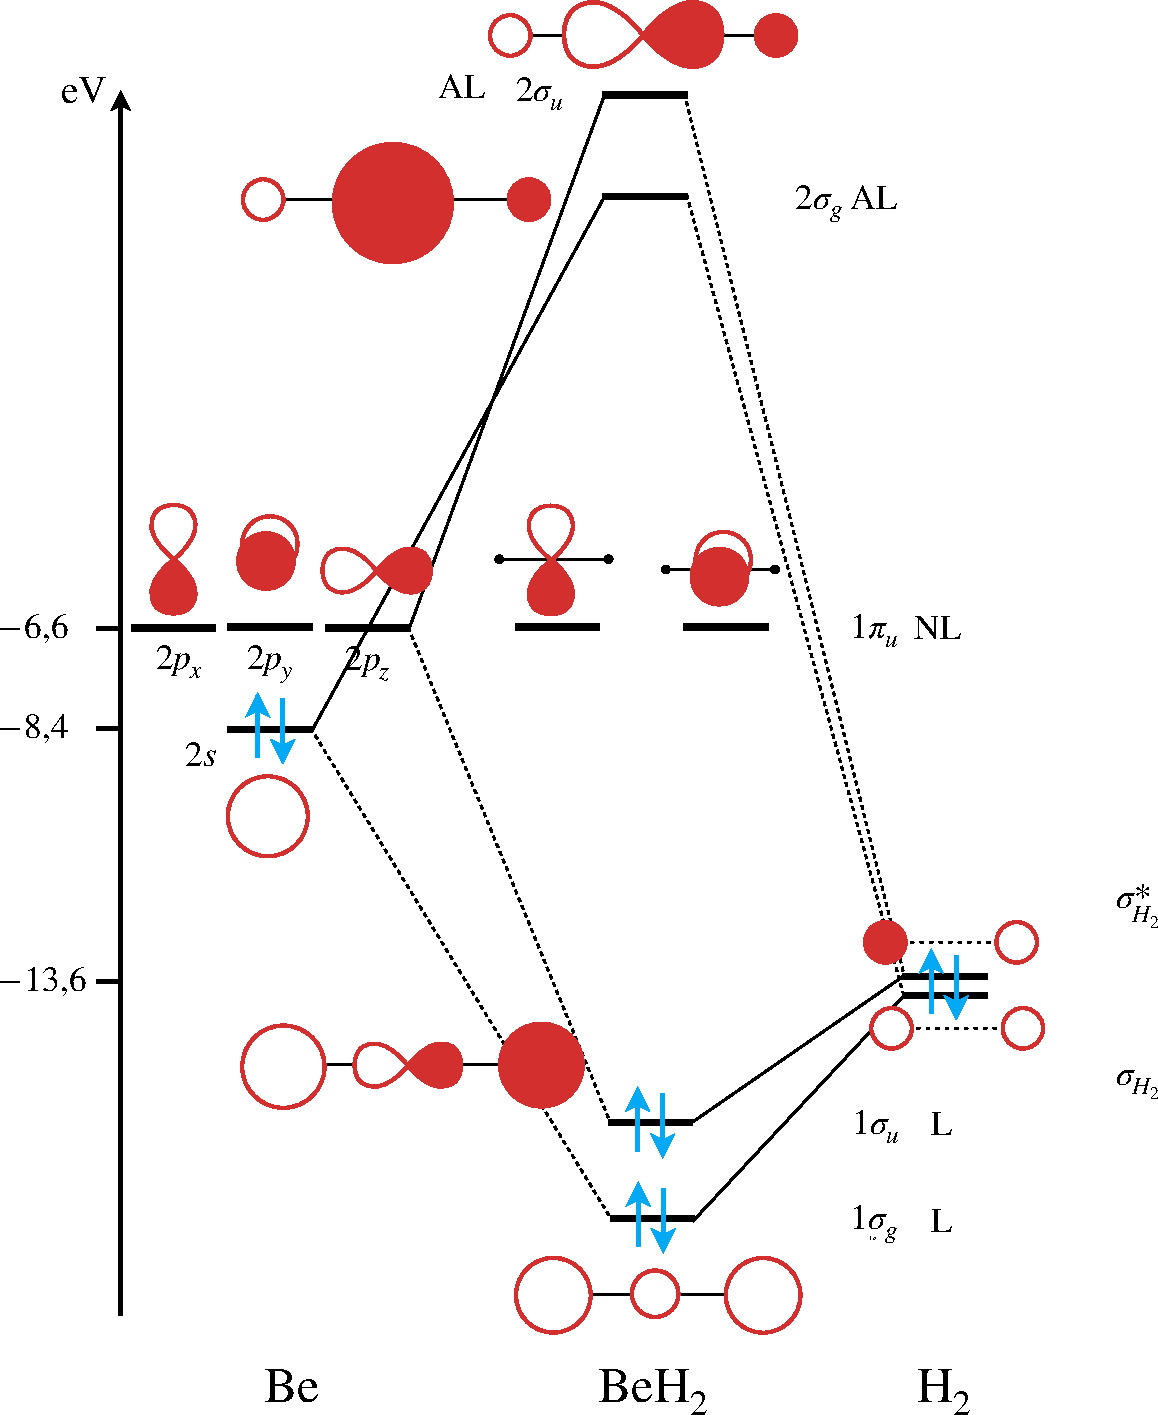
\includegraphics[scale=0.5]{figures/DOM_BeH2}

On fait de la m\^eme façon pour H2O\marginCritical{Ici, on n'a pas appliqué la règle des 15 eV afin d'obtenir un DOM exact.} :


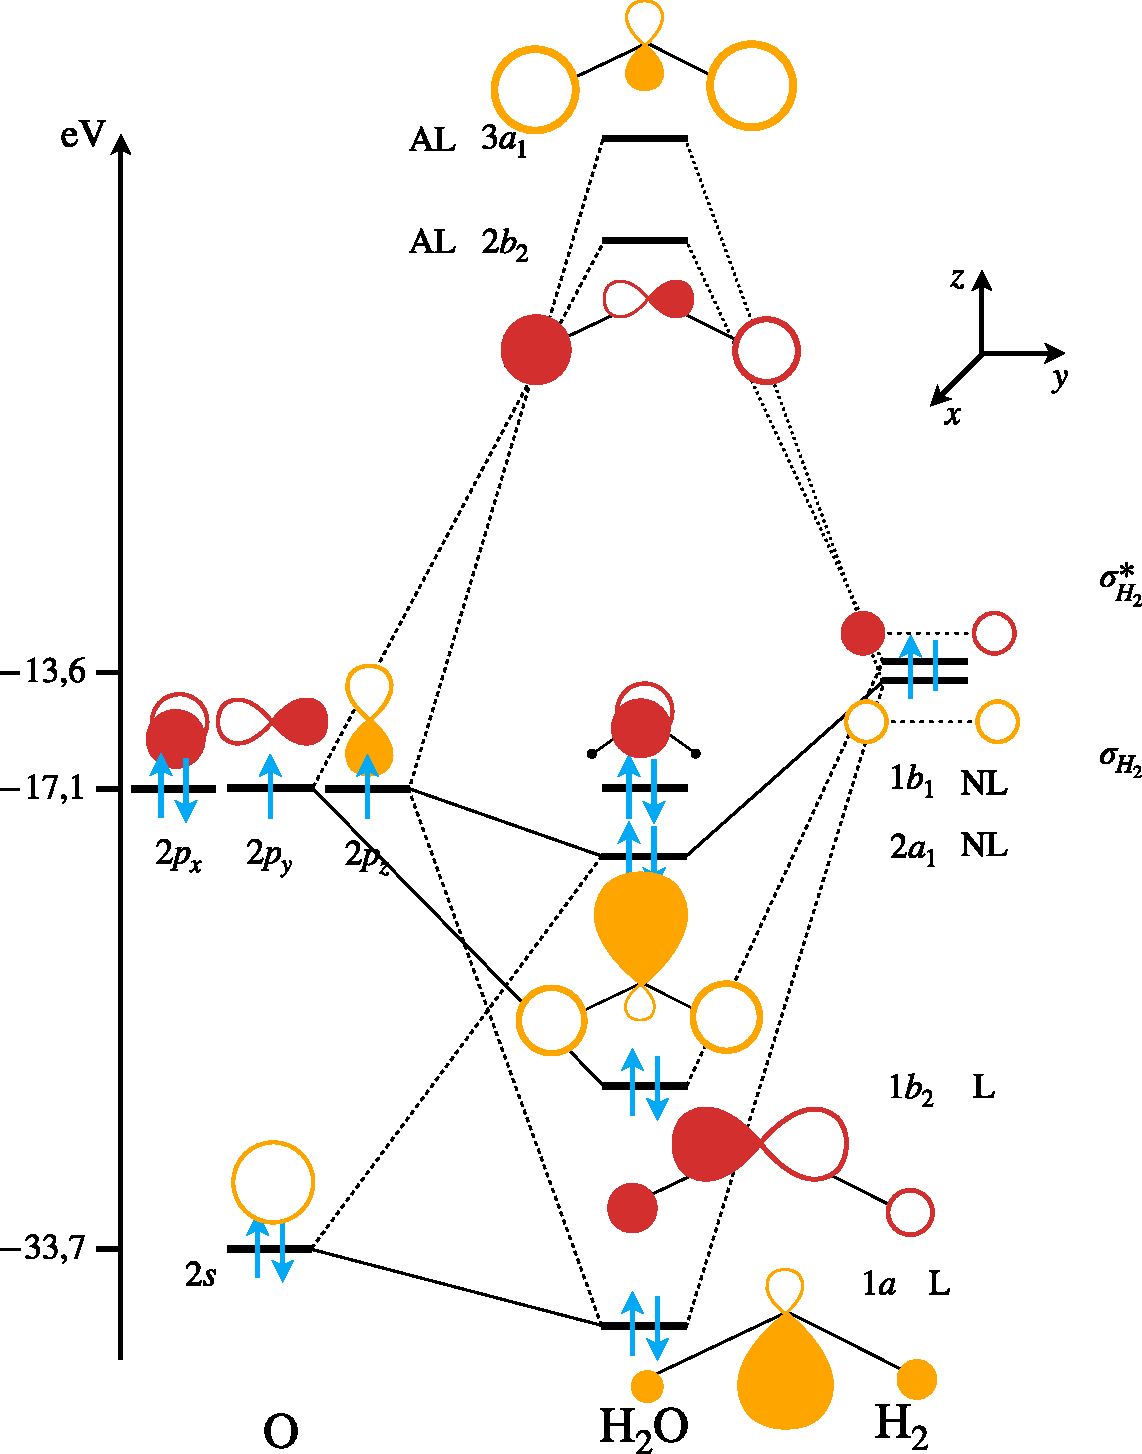
\includegraphics[scale=0.5]{figures/DOM_H2O}
\subsection{H3 Trigonal}
Il faut aussi savoir le digramme de \(H_3\) trigonal, qui peut servir pour des fragments à GPS de type DH par exemple.

 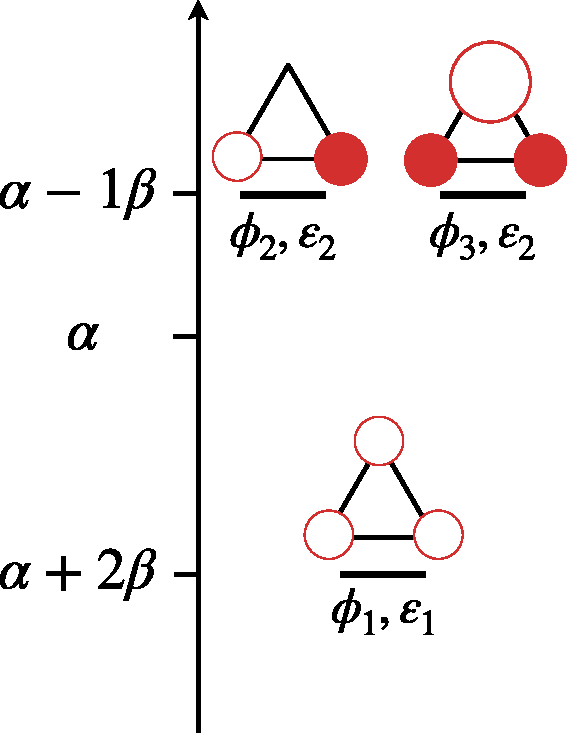
\includegraphics[scale=0.5]{figures/trigo.pdf}

\section{Interaction à 3 OA}


\includegraphics[scale=0.5]{figures/DOM_3OA}
 \end{document}
